\documentclass[a4paper,12pt]{article}
\usepackage{cmap}
\usepackage[utf8]{inputenc}
\usepackage[warn]{mathtext}
\usepackage{epsf,amsmath,amsfonts,amssymb,amsbsy}
\usepackage[mathscr]{eucal}
\usepackage[english, russian]{babel}
\author{Мещеряков Павел Б02-920}
\title{Отчёт о выполнении лабораторной работы 2.1.1}
\usepackage[left=2cm,right=2cm,top=2cm,bottom=2cm]{geometry}
\usepackage{graphicx}
\usepackage{indentfirst}
\graphicspath{{pictures2.1.1/}}
\DeclareGraphicsExtensions{.pdf,.png,.jpg}
\usepackage{pgfplots}
\begin{document}
	\maketitle
	\begin{center}
		{\Large Измерение удельной теплоёмкости воздуха при постоянном давленини}
	\end{center}
	\paragraph*{Цель работы:} измерить повышение температуры воздуха в зависимости от мощности
	подводимого тепла и расхода при стационарном течении через трубу; исключив тепловые потери, по результатам измерений определить теплоёмкость воздуха при постоянном давлении.
	\paragraph*{В работе используются:} теплоизолированная стеклянная трубка; электронагреватель; источник питания постоянного тока; амперметр, вольтметр (цифровые мультиметры); термопара, подключенная к микровольтметру; компрессор; газовый счётчик;
	секундомер.
	\section{Теоретическое введение}
	
		 Теплоёмкость тела в некотором процессе определяется как их отношение: $$ C = \frac{\delta Q}{dT} \; (1).$$
		 
		 Необходимо, чтобы количество тепла, затрачиваемое на нагревание исследуемого тела, существенно превосходило тепло, расходуемое на нагревание самого калориметра, а также на потери тепла из установки.
		 
		 Для увеличения количества нагреваемого газа при неизменных размерах установки в нашей работе исследуемый газ (воздух) продувается через калориметр, внутри которого установлен нагреватель. При этом
		 измеряются мощность нагревателя, масса воздуха, протекающего в единицу
		 времени (расход), и приращение его температуры.
		 
		 \begin{figure}[h]
		 \center{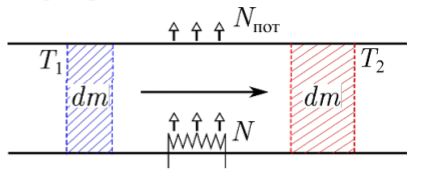
\includegraphics{lab_2_1_1}}
		 \end{figure}
		 Рассмотрим газ, протекающий
		 стационарно слева направо через
		 трубу постоянного сечения, в которой установлен нагревательный элемент (см. рис. 1). Пусть за некоторое
		 время $dt$ через калориметр прошла
		 малая порция газа массой $dm=q dt$,
		 где $q$ [кг/с] — массовый расход газа в трубе. Если мощность нагрева равна $N$, мощность тепловых потерь на обмен с окружающей средой $N_{пот}$, то порция
		 получила тепло $\delta Q = (N-N_{пот})dt$. С другой стороны, по определению теплоёмкости (1): $\delta Q = c dm \Delta T$, где $\Delta T = T_{2}-T_{1}$ — приращение температуры	газа, и $c$ — удельная (на единицу массы) теплоёмкость газа в рассматриваемом процессе. При малых расходах газа и достаточно большом диаметре
		 трубы перепад давления на её концах мал, поэтому можно принять, что $P_{1} \approx P_{2} = P_{0}$, где $P_{0}$ — атмосферное давление. Следовательно, в условиях опыта
		 измеряется удельная теплоёмкость при постоянном давлении $c_{P}$. Таким образом, получаем $$c_{P} = \frac{N-N_{пот}}{q\Delta T} \; (2).$$
		 
	\subsection{Эксперементальная установка:}
	
	Схема установки изображена на рис. 2. Воздух, нагнетаемый компрессором, прокачивается через калориметр. Калориметр представляет собой стеклянную цилиндрическую трубку с двойными стенками, запаянными с торцов.
	
		\begin{figure}[h]
		\center{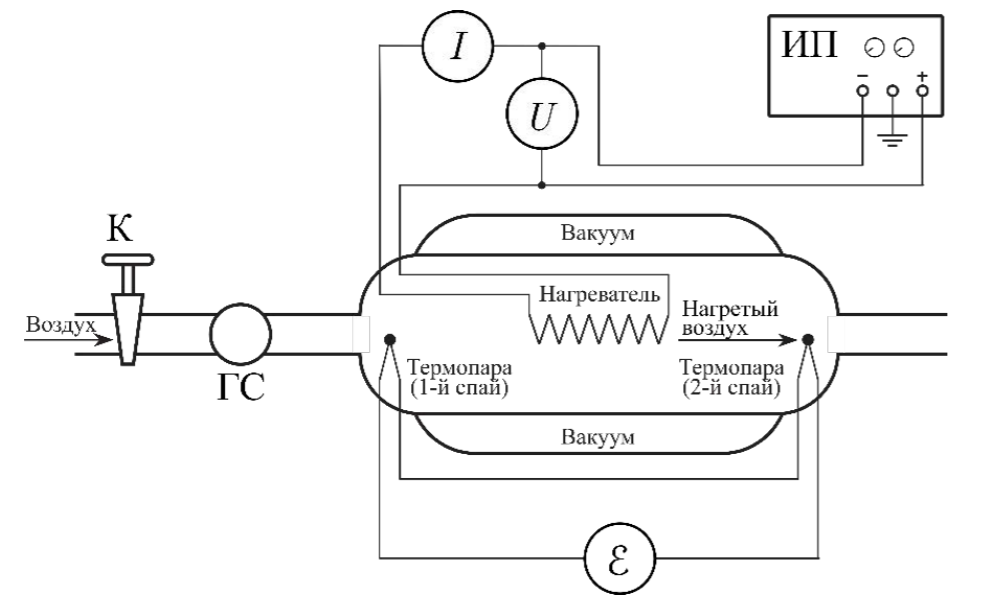
\includegraphics{lab_2_1_1_ust}}
		\end{figure}
	
		Нагреватель в виде намотанной на пенопласт нихромовой проволоки расположен внутри калориметра непосредственно в воздушном потоке. Нагрев проволоки производится от регулируемого источника постоянного тока (ИП).
		Напряжение $U$ на нагревателе и ток $I$ через него регистрируются цифровыми мультиметрами. Таким образом, мощность нагрева равна
		$$N= UI \; (3).$$ 
		Для измерения разности температур $\Delta T$ служит медно-константановая
		термопара. Один спай термопары расположен в струе воздуха, входящего в
		калориметр, и находится при комнатной температуре, а второй — в струе выходящего нагретого воздуха. Константановая проволока термопары расположена внутри калориметра, а медные проводники подключены к цифровому вольтметру. Возникающая в термопаре ЭДС $\varepsilon$ пропорциональна разности температур $\Delta T$ спаев: $$\varepsilon =\beta \Delta T \; (4),$$ где $\beta = 40.7 \frac{мкВ}{^\circ C}$ — чувствительность медно-константановой термопары в рабочем диапазоне температур (20–30 $^\circ C$ ). ЭДС регистрируется с помощью микровольтметра.
		
		Объём воздуха, прошедшего через калориметр, измеряется газовым счётчиком ГС. Для регулировки расхода служит кран К. Время $\Delta t$ прохождения
		некоторого объема $\Delta V$ воздуха измеряется секундомером. Объёмный расход равен $\frac{\Delta V}{\Delta t} $, массовый расход может быть найден как $$q = \rho_{0} \frac{\Delta V}{\Delta t} \; (5),$$ где $rho_{0}$ — плотность воздуха при комнатной температуре, которая в свою очередь может быть получена из уравнения Менделеева–Клапейрона: $\rho_{0}= \frac{\mu P_{0} }{R T_{0}},$ где $P_{0}$ — атмосферное давление, $T_{0}$ — комнатная температура (в Кельвинах), $\mu = 29,0 {г/моль}$ — средняя молярная масса (сухого) воздуха.
		
		Учитывая особенности устройства калориметра, следует ожидать, что мощность нагревателя расходуется не только на нагрев массы прокачиваемого воздуха, но и частично теряется за счет нагрева внутренних стенок термостата и рассеяния тепла через торцы термостата. Можно предположить, что при небольшом нагреве ($\Delta T \ll T_{0}$) мощность потерь тепла $N_{пот}$ прямо пропорциональна разности температур:$$ N_{пот} = \alpha \Delta T \; (6),$$ где $\alpha$ — некоторая константа. При этом условии основное соотношение (2) принимает вид $$N = (c_{P}q +\alpha)\Delta T \;(7)$$
		Следовательно, при фиксированном расходе воздуха ($q = const$ ) подводимая мощность и разность температур связаны прямой пропорциональностью($\Delta T(N)$ — линейная функция).
		
	\subsection{Ход работы}
	\begin{enumerate}
		\item Подготовим к работе газовый счетчик: проверим, что он заполнен  водой, установим счетчик по уровню.
		\item Охладим калориметр до комнатной температуры.
		\item Включим вольтметр, предназначенный для измерения ЭДС термопары. 
		\item Запишем показания компнатной температуры и давления. $$T_{0} = 297.05 \; ^\circ C, P_{0} = 99325 \pm 13 \; {Па} $$
		\item С помощью газового счетчика и секундомера измерим максимальный расход воздуха $\frac{\Delta V}{\Delta T}$ (в л/с). Измерения представлены в таблице 1. По найденным значениям определим среднее значение расхода и массовый расход воздуха $q_{max}$ [г/с].
		
		$$q = \rho_0 \frac{\Delta V}{\Delta t} = \frac{\mu P_0}{RT_0} \frac{\Delta V}{\Delta t}.$$
		
		Относительная погрешность косвенных измерений может быть найдена по формуле $$\frac{\sigma_{q_{max}кос}}{q_{max}} = \sqrt{(\frac{\sigma_{T_0}}{T_{0}})^2+(\frac{\sigma_{P_0}}{P_{0}})^2+ (\frac{\sigma_t}{t})^2}$$ 


	\begin{table}
	\begin{center}
	\begin{tabular}{|c|c|c|c|c|}
				\hline
				$\Delta V, л$ & $\Delta t, c$ & $\frac{\Delta V}{\Delta t},\frac{л}{с}$ & $q_{max},\frac{г}{c} $ & $\sigma_{q_{max}кос}, \; \frac{г}{с} \cdot 10^{-3}$ \\
				\hline
				5 & 25.68 & 0.1947 & 0.2272 & 1.769 \\
				\hline
				10 & 51.19 & 0.1953 & 0.2280 & 0.891\\
				\hline
				15 & 76.87 &  0.1951 & 0.2277 & 0.592\\
				\hline
				20 & 102.35 & 0.1954 & 0.2280 &0.446 \\
				\hline
				25 & 128.14 & 0.1951 & 0.2277 & 0.355\\
				\hline
				30 & 153.88 & 0.1950 & 0.2275 & 0.296 \\
				\hline
				35 & 179.58 & 0.1949 &0.2274 & 0.253 \\
				\hline
	
	\end{tabular}
	\end{center}
	\caption{Измерение расхода воздуха}
	\end{table}
	$$\overline{\frac{\Delta V}{\Delta t}} = 0.1951 \; \frac{л}{с} ,\; \overline{q_{max}} = 0.2276 \; \frac{г}{с} $$
	
	Случайная погрешность массового расхода может быть найдена по формуле: $$\sigma_{q_{max}сл} =  \sqrt{\frac{\sum_{i=1}^{7} (q_{max,i}-\overline{q_{max}})^2}{6}} = 0.0003 \; \frac{г}{c}.$$
	
	Косвенная погрещность для среднего значения: $q_{max}$ $$\sigma_{\overline{q_{max}}кос} = \sqrt{\frac{\sum_{i=1}^{7} (\sigma_{q_{max}кос})^2}{7^2}} = 0.0003 \; \frac{г}{c}.$$
	
	Суммарная погрешность: $$\sigma_{\overline{q_{max}}} = \sqrt{(\sigma_{q_{max}сл})+(\sigma_{\overline{q_{max}}кос})^2} = 0.0004 \; \frac{г}{c}.$$
	
	Окончательное значение: $$q_{max} = 0.2276 \pm 0.0004 \; \frac{г}{с} $$
	
	\item Оценим величину тока нагревателя $I_{0}$, требуемого для нагрева воздуха на $\delta T = 1 {К}$.
	
	Определим теоретическое значение удельной теплоемкости воздуха при постоянном давлении $C_{теорp} \; \frac{Дж}{г\cdot K}$, считая воздух смесью двухатомных идеальных газов: $Cp = 3.5R\mu \approx 1 \; \frac{Дж}{г\cdot K}.$
 	
 	Оценим минимальную мощность $N_0$, необходимую для нагрева газа при максимальном расходе. $N_{0} = c_{p}q\Delta T \approx 0.227 {Вт}.$
	
	Учитывая, что сопротивление проволоки нагревателя составляет приблизительно $R_{н} \approx 35 {Ом}$ и в процессе опыта практически не меняется, искомое значение тока $I_{0} = q N_{0} R_{н} \approx 0.08 \; {А}.$
	
	\item Проведем измерение зависимости разности температур от мощности нагрева $\Delta T(N)$ при максимальном расходе воздуха $q_0 = q_{max}.$
	\begin{table}

	\begin{center}
	\begin{tabular}{|c|c|c|c|c|c|c|c|c|}
		\hline
		$I, мA$ & $U, B$ & $N, Вт$ & $R_н, Ом$ & $\varepsilon, \muВ$ & $ \Delta T, K$
		\\
		\hline
		108.18 & 3.19 & 0.345 & 29.49 & 52 & 1.28 
		\\
		\hline
		141.62 & 4.18 & 0.592 & 29.52 & 88 & 2.16 
		\\
		\hline
		165.70 & 4.89 & 0.810 & 29.51 & 118 & 2.90 
		\\
		\hline
		181.06 & 5.34 & 0.967 & 29.49 & 141 & 3.46 
		\\
		\hline
		210.7 & 6.21 & 1.308 & 29.48 & 188 & 4.61 
		\\
		\hline
	\end{tabular}
	\end{center}
	\caption{Измерение $\Delta T (N) \; {при} \; q_{max}$}
	\end{table}
	Следует отметить, что погрешность измерения тока: $\sigma_{I} = 0.01 \; мA$, а  напряжения: $\sigma_{U}= 0.01 \; В$, $\sigma_{\varepsilon}= 1 \; \muВ$

	Завершив первую серию измерении, охладим калориметр до комнатнои температуры.
	Для этого отключим источник питания нагревателя, откроем кран К и продуем калориметр при максимальном расходе воздуха до тех пор, пока показания ЭДС не достигнут нуля.
	
	Данные представлены в таблице 2.
	
	\begin{table}
	\begin{center}
	\begin{tabular}{lr}
	\begin{tabular}{|c|c|c|c|c|}
	\hline
	$\Delta V, л$ & $\Delta t, c$  & $\frac{\Delta V}{\Delta t},\frac{л}{с}$ & $q_1, \frac{г}{c}$ & $Z, \; \frac{г}{с} \cdot 10^{-3}$ \\
	\hline
	5 & 46.02 & 0.1086 & 0.1266 & 0.550 \\
	\hline
	10 & 91.4 &  0.1094 & 0.1275 & 0.279 \\
	\hline
	15 & 134.78 & 0.1113 & 0.1297& 0.192 \\
	\hline
	20 & 178.96 & 0.1117 & 0.1302 & 0.146\\
	\hline
	25 & 221.14 & 0.1130 & 0.1317 & 0.119 \\
	\hline
	30 & 266.36 & 0.1126 & 0.1312 & 0.099\\
	\hline
	35 & 311.83 & 0.1122 & 0.1308 & 0.084\\
	\hline
	\end{tabular}
	
	\begin{tabular}{|c|c|c|c|c|}
	\hline
	$\Delta V, л$ & $\Delta t, c$  & $\frac{\Delta V}{\Delta t},\frac{л}{с}$ & $q_2, \frac{г}{c}$ & $Z, \; \frac{г}{с} \cdot 10^{-3}$ \\
	\hline
	1 & 13.40 & 0.0747 & 0.0870 & 1.30\\
	\hline
	2 & 27.56 & 0.0726 & 0.0846 & 0.61\\
	\hline
	3 & 41.31 & 0.0726 & 0.0846 & 0.41\\
	\hline
	4 & 54.95 & 0.0733 & 0.0855 & 0.31 \\
	\hline
	5 & 69.05 & 0.0724 & 0.0844 & 0.24\\
	\hline
	6 & 82.24 & 0.0729 & 0.0850 & 0.21\\
	\hline
	7 & 96.18 & 0.0728 & 0.0848 & 0.18 \\
	\hline
\end{tabular}
\end{tabular}
\end{center}
\caption{Измерения других расходов; $q_1 = 0.123  \pm 0.002 \; \frac{г}{с}; \; q_2 = 0.085 \pm 0.001 \; \frac{г}{с} $ }
\end{table}
	Проведем аналогичные измерения для других значений расхода воздуха. Новая температура $T_{0} = 297.4 ^\circ C$.
	Данные представлены в таблице 3 и 4.  ($Z \equiv \sigma_{q_{max}кос}$). Погрешности рассчитаны аналогично $q_{max}.$

\begin{table}
	\begin{center}
		\begin{tabular}{lr}
			\begin{tabular}{|c|c|c|c|c|c|}
				\hline
				$I, A$ & $U, B$ & $N, Вт$ & $R_н, Ом$ & $\varepsilon, \muВ$ & $ \Delta T, K$\\
				\hline
				91.34 & 2.69 & 0.246 & 29.45 & 50 & 1.23 \\
				\hline
				120.30 & 3.55 & 0.427 & 29.51 & 89 & 2.19 \\
				\hline
				145.11 & 4.28 & 0.621 & 29.49 & 128 & 3.14 \\
				\hline
				176.45 & 5.20 & 0.918 & 29.47 & 184 & 4.52 \\
				\hline
				212.20 & 6.23 & 1.322 & 29.36 & 261 & 6.41 \\
				\hline	
			
			\end{tabular}
			\begin{tabular}{|c|c|c|c|c|c|}
				\hline
				$I, A$ & $U, B$ & $N, Вт$ & $R_н, Ом$ & $\varepsilon, \muВ$ & $ \Delta T, K$\\
				\hline
				105.95 & 3.13 & 0.332 & 29.54 & 81 & 1.99 \\
				\hline
				125.74 & 3.71 & 0.466 & 29.51 & 128 & 3.14 \\
				\hline
				149.46 & 4.41 & 0.659 & 29.50 & 175 & 4.30 \\
				\hline
				177.33 & 5.23 & 0.927 & 29.49 & 236 & 5.80 \\
				\hline
				211.5 & 6.25 & 1.322 & 29.55 & 310 & 7.62 \\
				\hline
			\end{tabular}
		\end{tabular}
	\end{center}
	\caption{Измерение $\Delta T (N) \; {при} \; q_{1} \; и \; q_{2}$}
\end{table}

		Погрешности будем считать по слудующим формулам: $$ \sigma_{\Delta T} = \Delta T \frac{\sigma_{\varepsilon}}{\varepsilon}, \sigma_{N}= N\sqrt{( \frac{\sigma_{I}}{I})^2 + (\frac{\sigma_{U}}{U})^2} \approx N \frac{\sigma_{U}}{U}$$
	
		\begin{table}
		\begin{tabular}{lr}
		\begin{tabular}{|l|l|l|l|l|l|l|l|l|l|l|}
			\hline
			q, $\frac{г}{с}$ & \multicolumn{4}{|c|}{0.2276} & \multicolumn{4}{|c|}{0.123}
			\\
			\hline
			k &  $\Delta T, \; ^\circ C$& $\sigma_{\Delta T}\; ^\circ C$ & $N$, мВт & $\sigma_{N}$, мВт & $\Delta T, \; ^\circ C$& $\sigma_{\Delta T}\; ^\circ C$ & $N$, мВт & $\sigma_{N}$, мВт
			\\
			
			\hline
			0 & 0 & 0 & 0 & 0 & 0 & 0 & 0 & 0
			\\
			\hline
			1 & 1.28 & 0.02 & 345 & 1.1 & 1.23 &  0.02 & 246 & 0.9
			\\
			\hline
			2 & 2.16 & 0.02 & 592 & 1.4 & 2.19 & 0.02 & 427 & 1.2
			\\
			\hline
			3 & 2.90 & 0.02 & 810 & 1.7 & 3.14 & 0.02 & 621 & 1.5
			\\
			\hline
			4 & 3.46 & 0.02 & 967 & 1.8 & 4.52 & 0.02 & 918 & 1.8
			\\
			\hline
			5 & 4.61 & 0.02 & 1308 & 2.1 & 6.41 & 0.02 & 1322 & 2.1
			\\
			\hline
		\end{tabular}

		\\

		\begin{tabular}	{|l|l|l|l|l|l|l|l|l|l|l|}
		\hline
		q, $\frac{г}{с}$ & \multicolumn{4}{|c|}{0.085} 
		\\
		\hline 
		k &  $\Delta T, \; ^\circ C$& $\sigma_{\Delta T}\; ^\circ C$ & $N$, мВт & $\sigma_{N}$, мВт
		\\
		\hline
		0 & 0 & 0 & 0 & 0
		\\
		\hline
		1 & 1.99 & 0.02 & 332 & 1.1 
		\\
		\hline
		2 & 3.14 & 0.02 & 466 & 1.3 
		\\
		\hline
		3 & 4.30 & 0.02 & 659 & 1.5 
		\\
		\hline
		4 & 5.80 & 0.02 & 927 & 1.8
		\\
		\hline
		5 & 7.62 & 0.02 & 1322 & 2.1
		\\
		\hline	
	\end{tabular}



		\end{tabular}
	\caption{ погрешности, $\Delta T \; и \; N$}
	\end{table}


	После завершения опытов выключим источник питания нагревателя и мультиметры. Кран К откроем для максимального продува воздуха через калориметр.
	
\item Построим на одном графике зависимости $\Delta T (N)$ при разных значениях $q$.
	\begin{center}
			\begin{tikzpicture}[scale = 2]
			\begin{axis}[
			axis lines = left,
			legend style={at={(1,0.3)}},
			xlabel = {$N$, {мВт}},
			ylabel = {$\Delta T, {^\circ C} $
			},
			xmin=0, xmax=1350,
			ymin=0, ymax=8,
			ymajorgrids = true,
			xmajorgrids = true,
			minor tick num = 4
			]
			\addplot+[only marks ] plot[error bars/.cd, y dir=both, y explicit]
			coordinates {
				(0,0)
				(345,1.28) 
				(592, 2.16)
				(810, 2.90)
				(967 , 3.46)
				(1308, 4.61)
			};
			\addplot+[only marks ] plot[error bars/.cd, y dir=both, y explicit] coordinates {
				(0,0)
				(246,1.23) 
				(427, 2.19)
				(621, 3.14)
				(918 , 4.52)
				(1322, 6.41)
			};	
			\addplot+[only marks ] plot[error bars/.cd, y dir=both, y explicit]
			coordinates {
				(0,0)
				(332,1.99) 
				(466, 3.14)
				(659, 4.30)
				(927 , 5.80)
				(1322, 7.62)
			};
		

			\addplot[blue, domain=0:1350]{0.042+0.0035*x};
			\addplot[red, domain=0:1350]{0.0619+0.0048*x};
			\addplot[brown, domain=0:1350]{0.0210+0.0063*x};
			\legend{
				$q_{max} = 0.2276 \frac{г}{с}$, $q_{1} = 0.123 \frac{г}{с};$ , $ q_{2} = 0.085 \frac{г}{с};$
			};
 			\end{axis}
			\end{tikzpicture}
		\end{center}
		${y_{max} = (3.5 \pm 0.3 )10^{-3}x+0.042 \pm 0.027}$,\\
		$\; {y_{1} = (4.8 \pm 0.1)10^{-3}x+0.062 \pm 0.044}$,\\
		$\; {y_{2} = (6.3 \pm 0.2)10^{-3}x+0.021 \pm 0.12}.$
		$Чтобы \; найти \; k_{max},\; k_1, \; k_2$, необходимо перевернуть соотвествующие коэффициенты $k'$ наклонов прямых, а погрешность считать по формуле: $$\sigma_k = k^2 \sigma_{k'}.$$
		$k_{max} = 0.286 \pm 0.025 \; \frac{Вт}{К}, \; k_{1} = 0.208 \pm 0.004 \; \frac{Вт}{К}, \; k_{2} = 0.159 \pm 0.005 \; \frac{Вт}{К} $

		Прямая для расхода $q_2$ не идёт из нуля, вероятно, из-за поспешного начала третей серии измерений (начальная температура была несколько больше комнатной). Однако в целом из вида наших прямых, можно сделать вывод о том, что тепловые потери пропорциональны разности температур.

	
		Построим график зависимости $k(q)$ и по его наклону определим теплоёмкость воздуха при постоянном давлении $c_p$
		
		\begin{center}
		\begin{tikzpicture}[scale = 1]
		\begin{axis}[
		axis lines = left,
		legend style={at={(1,1)}},
		xlabel = {$q, \; \frac{г}{с} \cdot 10^{-1}$},
		ylabel = {$k, \frac{Вт}{К}$
		},
		xmin=0, xmax=3,
		ymin=0, ymax=0.5,
		ymajorgrids = true,
		xmajorgrids = true,
		minor tick num = 4
		]
		\addplot+[only marks ] plot[error bars/.cd, x dir=both, x explicit ,y dir=both, y explicit]
		coordinates {
			(2.276,0.286) +- (0.004,0.025)
			(1.23, 0.208 ) +- (0.02,0.004)
			( 0.85,0.159) +- (0.01,0.005)
		};
		\addplot [red, domain=0:3]{0.0928+0.0860*x};
		
		\legend{
			$$y=0.0928+0.0860x$$
		};
		\end{axis}
		\end{tikzpicture}
		\end{center}
	
Итак, из графика найдём $c_p = (0.86 \pm 0.1) \; \frac{Дж}{К \cdot г} \cdot 29 \frac{г}{моль} = 24.94 \pm 2.29 \; \frac{Дж}{К моль}.$ A также $\alpha = 0.093 \pm 0.018 \; \frac{Вт}{К}.$ К сожалению, теплоёмкость значительно отличается от теоретического значения $29.09 \; \frac{Дж}{К моль}.$ Измерения необходимо было проводить более тщательно, ждать установления термодинамического равновесия более длительное время. Однако не смотря на это, результаты, полученные при обработке данных совпадают (почти) с теоретическими с учётом погрешностей.

Посчитаем доли тепловых потерь в опытах : $\frac{N_{пот}}{N} =\frac{\alpha}{k}$

	\begin{center}
	\begin{tabular}{|c|c|}
		\hline
		$q, \; \frac{г}{с}$ & $\frac{N_{пот}}{N}$ \\
		\hline
		0.085 & $0.59 \pm 0.11$ \\
		\hline
		0.123 & $0.45 \pm 0.09$\\
		\hline
		0.2276 & $0.33 \pm 0.06$ \\
		\hline
	\end{tabular}
	\end{center}

\end{enumerate}

\end{document}